%\sectskip
\vspace{-5pt}
\section{Layers with Environment Context}
\label{sec:machine}


\begin{figure}
\begin{center}
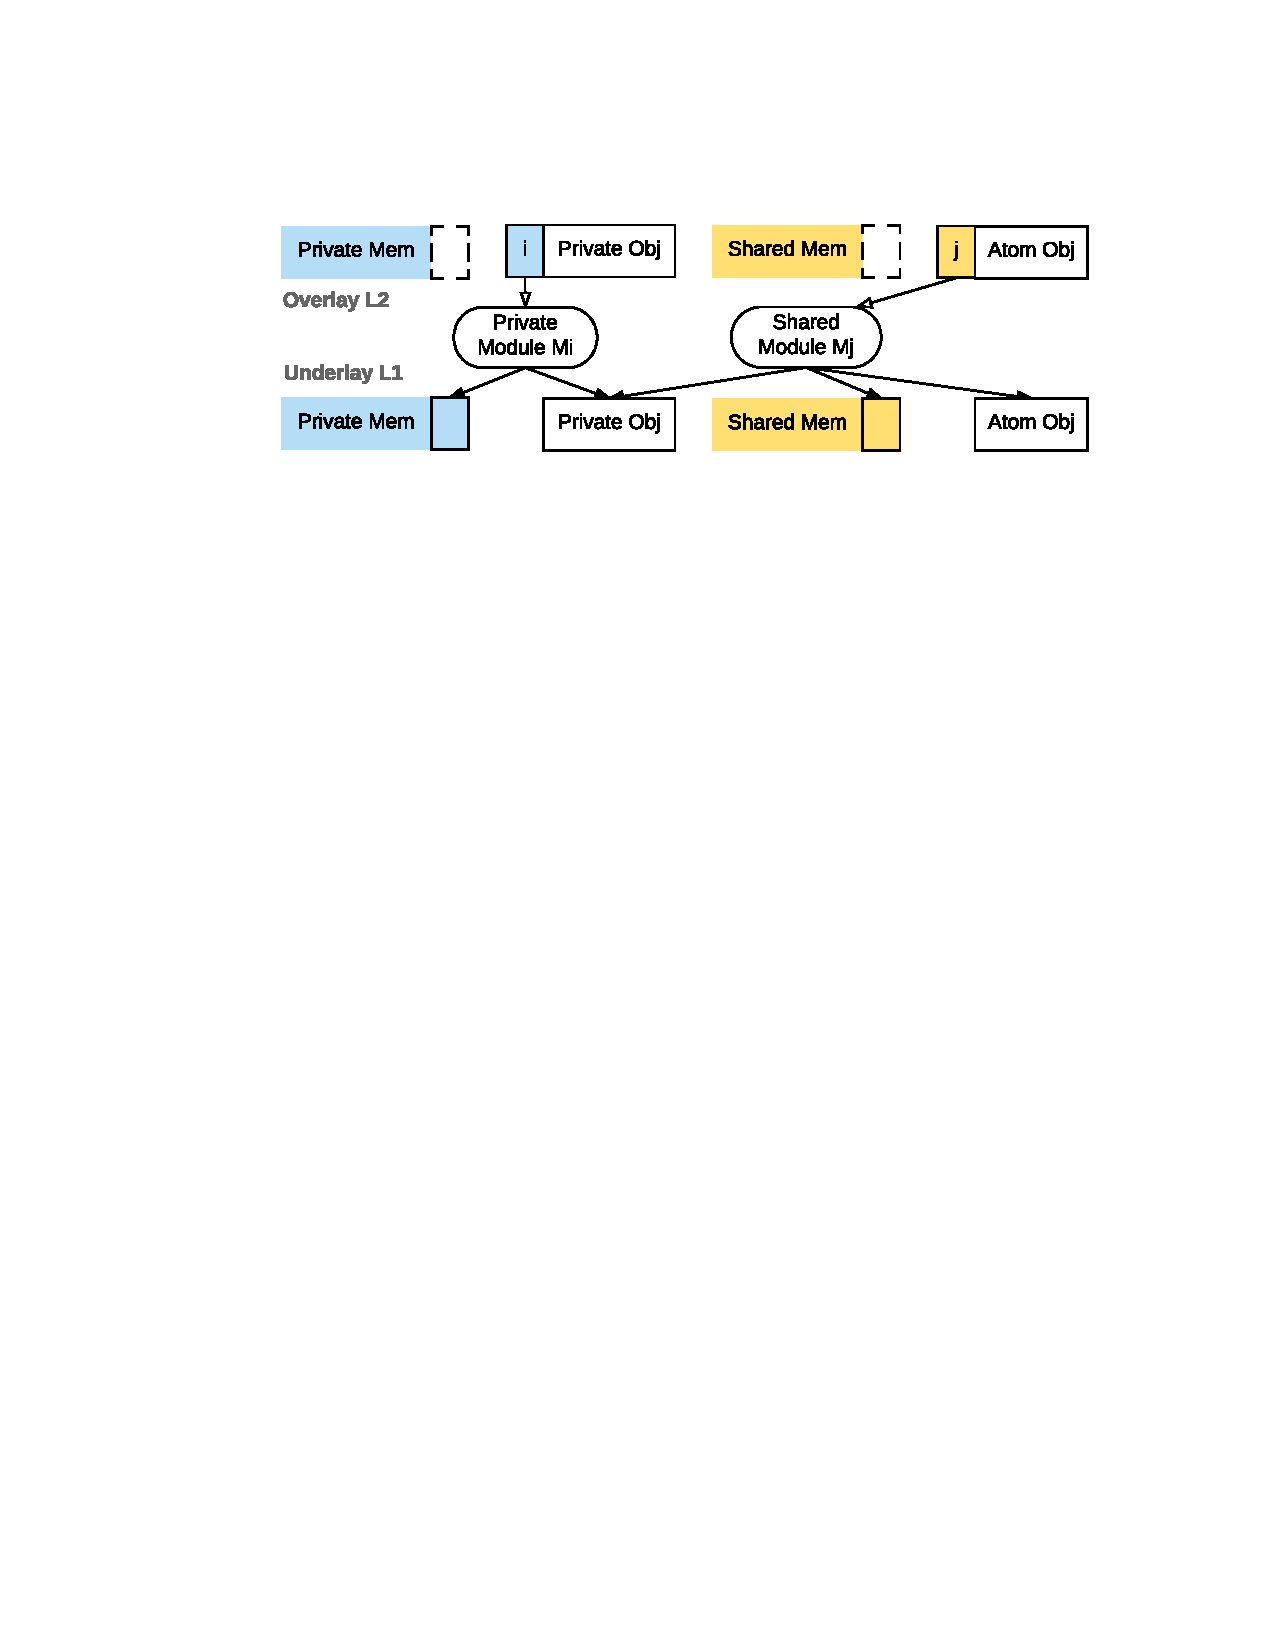
\includegraphics[scale=0.55]{figs/build_object}
\vspace*{-8pt}	
\end{center}
\caption{Defining concurrent abstraction layers.}
\label{fig:spec:object}
\vspace*{-10pt}
\end{figure}


In this section, we explain the general layer design principles and present
how we use environment context to convert a concurrent layer into 
 CPU-local layers.
\ignore{that is suitable for reasoning about concurrent code in a CPU-local way.}

\vspace*{-3pt}
\paragraph{Multicore hardware} allows
all the CPUs to access the same piece of memory
simultaneously.
In {\CTOS}, we \emph{logically} distinguish the \emph{private memory} 
(\ie, private to a CPU or a thread) from the \emph{shared memory} 
(\ie, can be accessed by multiple CPUs or threads). 
The private memory does not
need to be synchronized, whereas non-atomic
shared memory accesses need to be protected by some synchronization mechanisms
(\eg, locks), which are normally implemented using atomic hardware instructions
(\eg, fetch-and-add). With proper protection,
each shared memory operation can be viewed as if it were atomic.

\vspace*{-3pt}
\paragraph{Atomic object}
\ignore{In {\CTOS}, we refine each piece of shared data with well synchronized operations
into an \emph{atomic object}. An atomic object}

is an abstraction of well-synchronized shared memory, combined
with operations that can be performed over that shared memory.
It consists of a set of
primitives, an initial state, and a \emph{logical log} containing the entire
history of the operations that were performed on the object during
an execution. Every primitive invocation
records a \emph{single} corresponding event in the log. 
We require that these events contain enough information to derive the
current state of an atomic object by replaying the entire log starting 
from the object's initial state.
\ignore{ 
Note that every atomic primitive at the overlay always generates
exactly one event (this is how we make sure that it is really atomic),
while the actual implementation may trigger multiple events (by
calling multiple atomic primitives at underlay). The events are are
shuffled and merged during the contextual refinement, which we explain
in more detail in the subsequent subsections.
}

\vspace*{-3pt}
\paragraph{Concurrent layer interface}
$L$ is a collection of both \emph{private objects} and \emph{atomic objects},
along with some invariants imposed on these objects.
The verification of a concurrent kernel 
requires repeatedly 
building certified abstraction layers $(L_1, M, L_2)$.
The overlay interface $L_2$ is a
new and more abstract interface
built upon the underlay interface $L_1$ using module $M$
 (\cf Fig.~\ref{fig:spec:object}).
\emph{Private objects} are built from private modules with 
only private memory accesses
using techniques similar to those presented by Gu {\it et al} \cite{dscal15}. 
\emph{Atomic objects} are built from the 
existing atomic objects, private objects,
and modules with non-atomic shared memory accesses.

\ignore{
The framework requires the defined invariants to hold at any point in
the program execution. Invariant proofs are found to be particularly
challenging even in the sequential setting, where in many cases,
some invariants are temporarily violated and re-established later \cite{klein2009sel4}.
In {\CTOS}, thanks to our layered approach, we can impose different invariants
at different abstraction layers. The primitives at underlay can be hidden if they
are no longer needed at overlay, such that stronger invariants can be introduced
at some overlay with atomic primitives, which could otherwise be violated by the
lower-level primitives at underlays.
}

\ignore{
\paragraph{Verification task}
The major task to verify a concurrent kernel
is to show that kernel modules with shared memory accesses
have atomic interfaces.
In other words, the verification of a concurrent kernel
is a procedure to 
build new atomic objects based on the 
existing atomic objects, private object,
and non-atomic shared data
(\cf Fig.~\ref{fig:spec:object}).}
 
\vspace*{-3pt}
\paragraph{Verification task}
It is difficult to build certified abstraction layers
directly on
a multicore, nondeterministic hardware model. To build an atomic object,
one must reason about all of the unnecessary interleavings (\eg, the interleavings
between private operations), and prove that every access to shared memory is
well synchronized. Furthermore, it is not clear how we can reason about threads
running on each core locally and combine the proofs to obtain a global claim about the whole system.

In the remainder of this section, we first present our x86 multicore machine model
($\mach{x86mc}$), and then show how we gradually refine this low-level model into a
more abstract machine model ($\mach{loc}$) that is suitable
for reasoning about concurrent code in a CPU-local fashion.

\begin{figure*}
\begin{center}
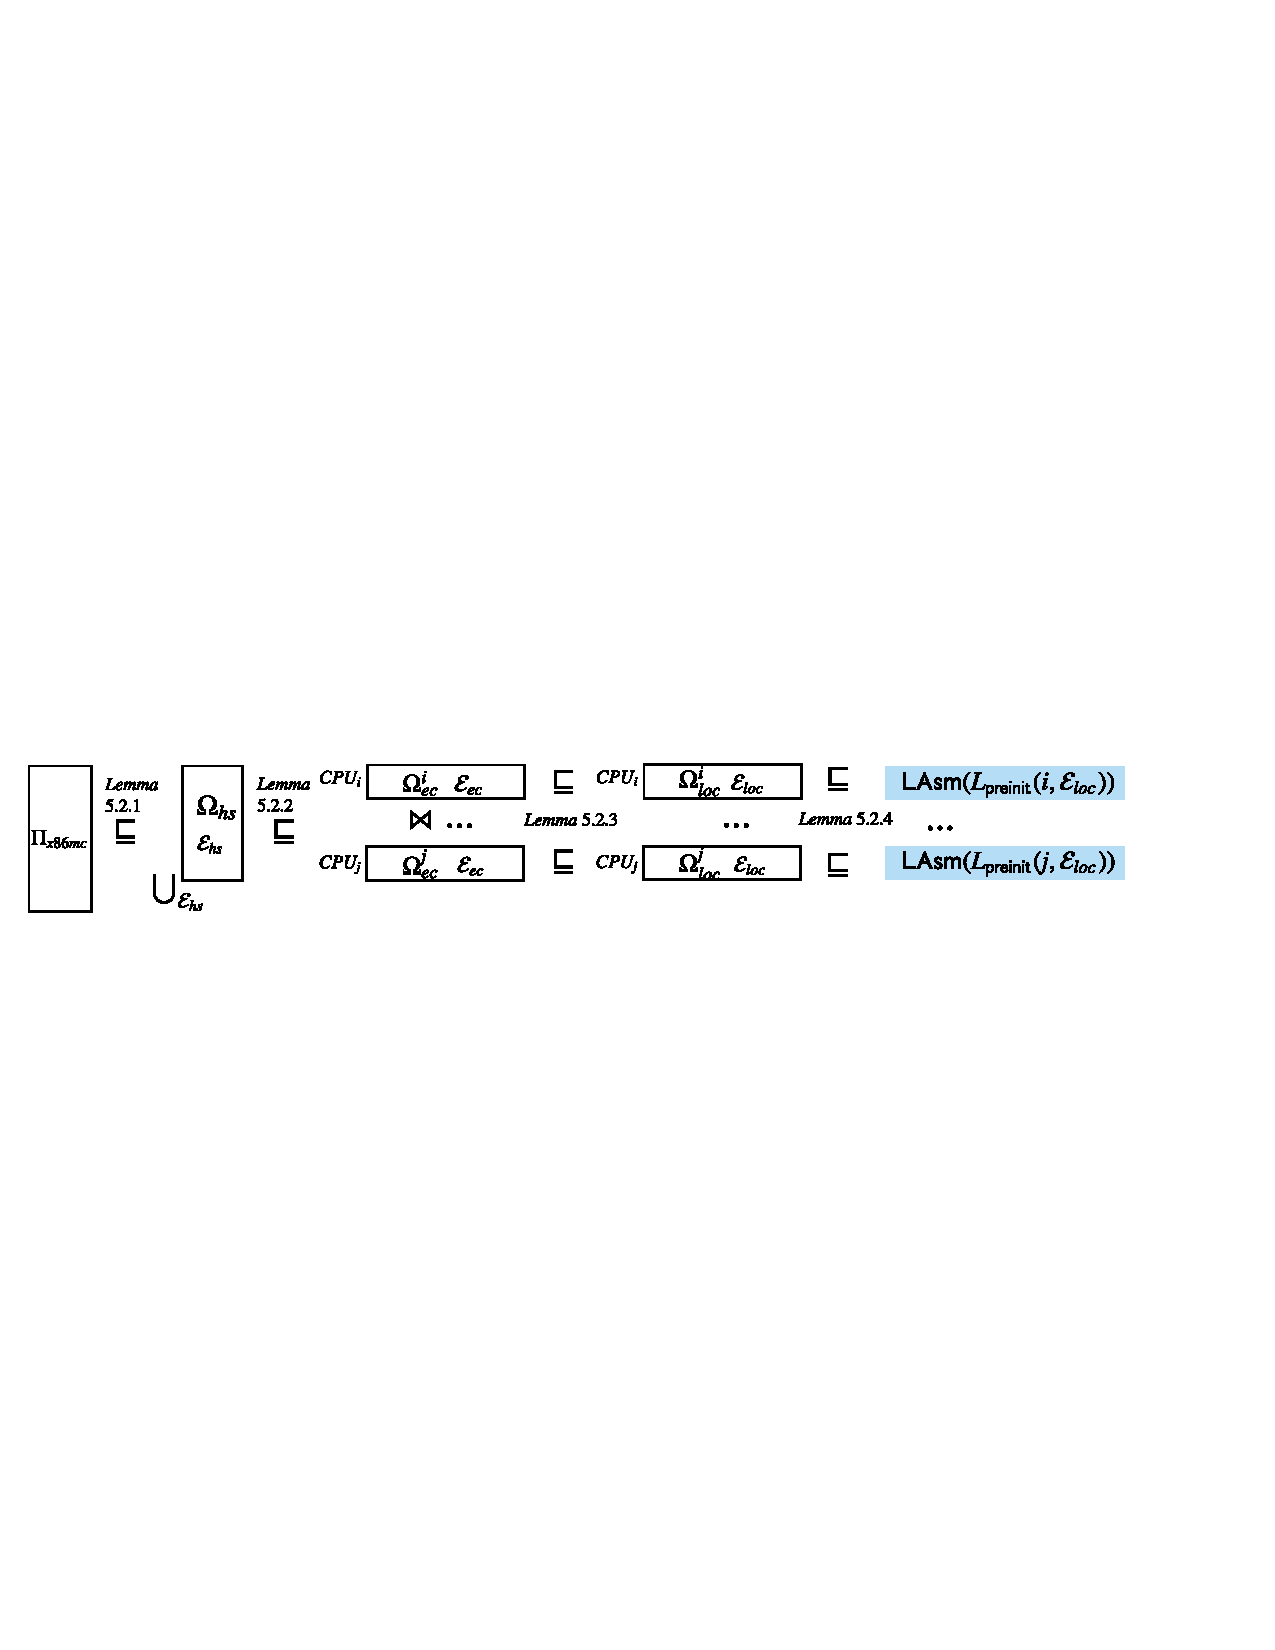
\includegraphics[scale=0.8]{figs/machine_chain}
\vspace*{-8pt}	
\end{center}
\caption{The contextual refinement chain from multicore hardware model
$\mach{x86mc}$ to CPU-local model $\mach{loc}$.}
\label{fig:spec:chain}
\vspace*{-10pt}
\end{figure*}

\vspace*{-2pt}
\subsection{Multicore hardware model}
Our fine-grained multicore hardware model ($\mach{x86mc}$) allows arbitrary
interleavings at the level of \emph{assembly instructions}.
At each step, the hardware \emph{randomly} chooses one CPU 
and executes the next assembly instruction on that CPU.
Each assembly instruction is classified as \emph{atomic}, \emph{shared},
or \emph{private}, based on if it involves an atomic object call,
a  non-atomic shared memory access, or only a private 
object/memory access.
One interleaving of an example program running on two CPUs
is:\vspace{-5pt}
\[
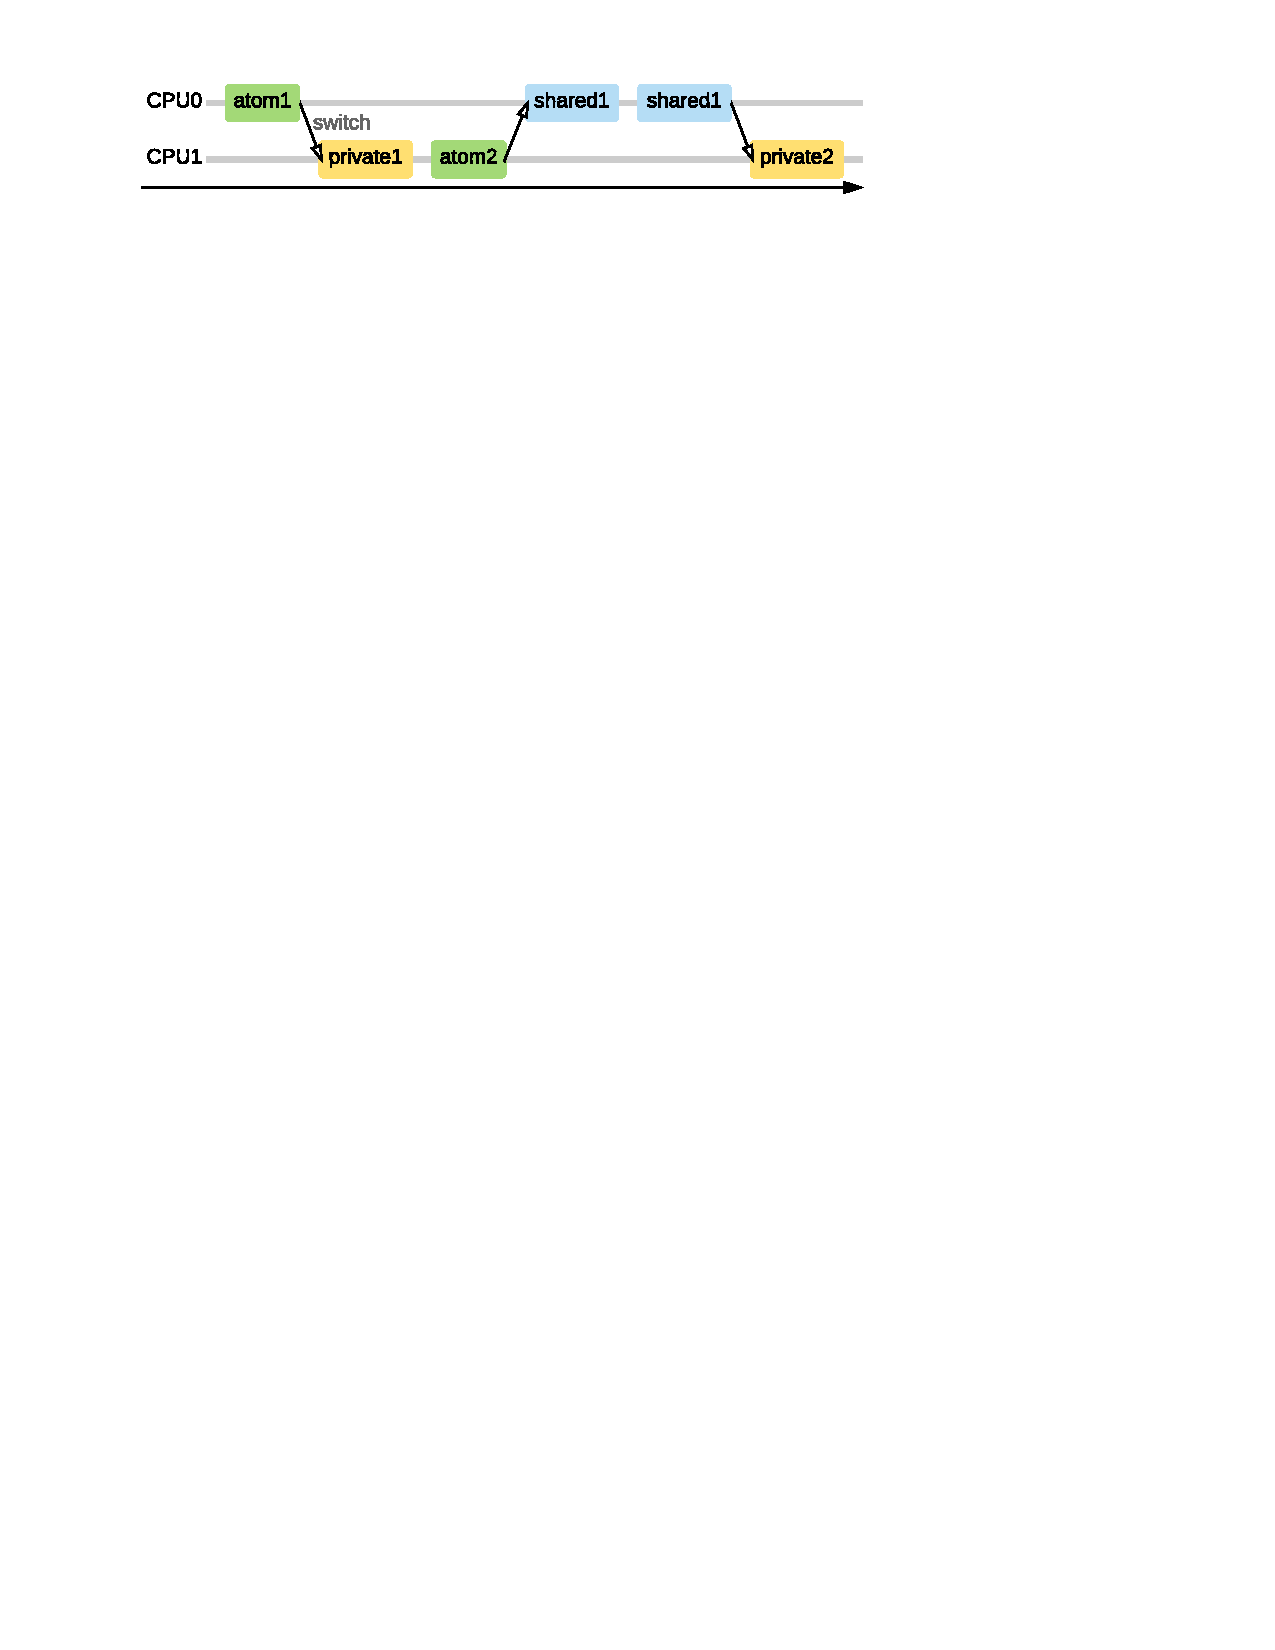
\includegraphics[scale=.65]{figs/machine1}
\vspace{-5pt}
\]
Since only atomic operations generate events,
this interleaving produces the logical log $[\event{0.atom_1,1.atom_2}]$.
\ignore{
Note that, while we mentioned above that each atomic object has its own
logical log, our model will actually maintain only a single log throughout an
execution. To obtain a per-object log, one can simply ignore all events in the
log that do not pertain to the desired atomic object.}

\ignore{
\paragraph{Memory model}
\ignore{
\ronghui{Maybe we do not need to talk about Compcert memory model?}
Because we use CompcertX~\cite{dscal15} along with
its formalization of the semantics of C and assembly,
our notion of memory is based on the CompCert memory model~\cite{leroy08}.
CompCert employs a unified model
to encode different views of memory.
The memory is split into a number of disjoint blocks and
a pointer is represented by a pair $(b, o)$, where
$b$ is a block identifier and
$o$ is an offset within block $b$.
Each offset within a block is associated with a permission
specifying the memory operations that can be performed at that location.
A program which attempts to perform a prohibited operation will \emph{get stuck}.
}

We \emph{logically} divide the machine memory into three parts:
\emph{atomic object}, \emph{shared memory},
and \emph{private memory}.
An \textbf{atomic object}
is accessed only through atomic operations
(\eg, compare-and-swap) provided by the hardware. Since these atomic operations
(denoted as \code{atom\_op})
are expensive, they are only used to implement the synchronization mechanisms
(\eg, locks). In our hardware model, each atomic operation generates 
\emph{exactly one event} that is recorded in a 
list of atomic events called a \emph{logical log}.
As shown in the ticket lock example \ronghui{reference?},
both \emph{ticket} and \emph{now} fields belong to the atomic object
and their operations generate the events $\event{inc\_ticket}$
and $\event{get\_now}$. Each method on the atomic object is considered
as atomic (as specified in the hardware manual) and its interface
is represented as a single
event. The values of an atomic object can be reconstructed from its logical log. 
\newman{I assume the events, log, and replay functions will be defined somewhere
in the Overview section?}

Operations to access shared memory and private memory
are denoted as \code{shared\_op} and \code{private\_op}, respectively.
Distinguishing between these makes it easier to reason about CPU-local 
execution.


\paragraph{Building atomic objects}
Shared memory accesses are not atomic. 
To ensure safety of the kernel,
shared memory has to be protected by synchronization
methods implemented using atomic objects.
The main task when verifying shared modules is to show that
each operation over shared memory can be viewed as if it were
atomic, provided the access is well synchronized by the atomic objects.
Therefore, concurrent kernel verification can be viewed as a procedure
to build concurrent objects with atomic interfaces (\cf Sec.~\ref{subsec:layer_def}).

\paragraph{Interleaving semantics}
}

\vspace*{-2pt}
\subsection{Machine model with hardware scheduler}
As a first step toward abstracting away the low-level details of
concurrent CPUs, we introduce a new machine model ($\mach{hs}$) configured
with a
\emph{hardware scheduler} ($\hardoracle$) that specifies a 
particular interleaving for an execution. 
This results in a deterministic machine model.
To take a program from $\mach{x86mc}$ and run it on top of $\mach{hs}$,
we insert a  \emph{logical \intptext}
(denoted as ``$\intp$") before each assembly instruction.
At each \intptext, the machine first queries the hardware scheduler
and gets the CPU ID to execute next.
All the \emph{switch decisions} made by $\hardoracle$ are stored in the 
log as switch events. 
The previous example on $\mach{x86mc}$
can be simulated by the following $\hardoracle$:\vspace{-5pt}
\[
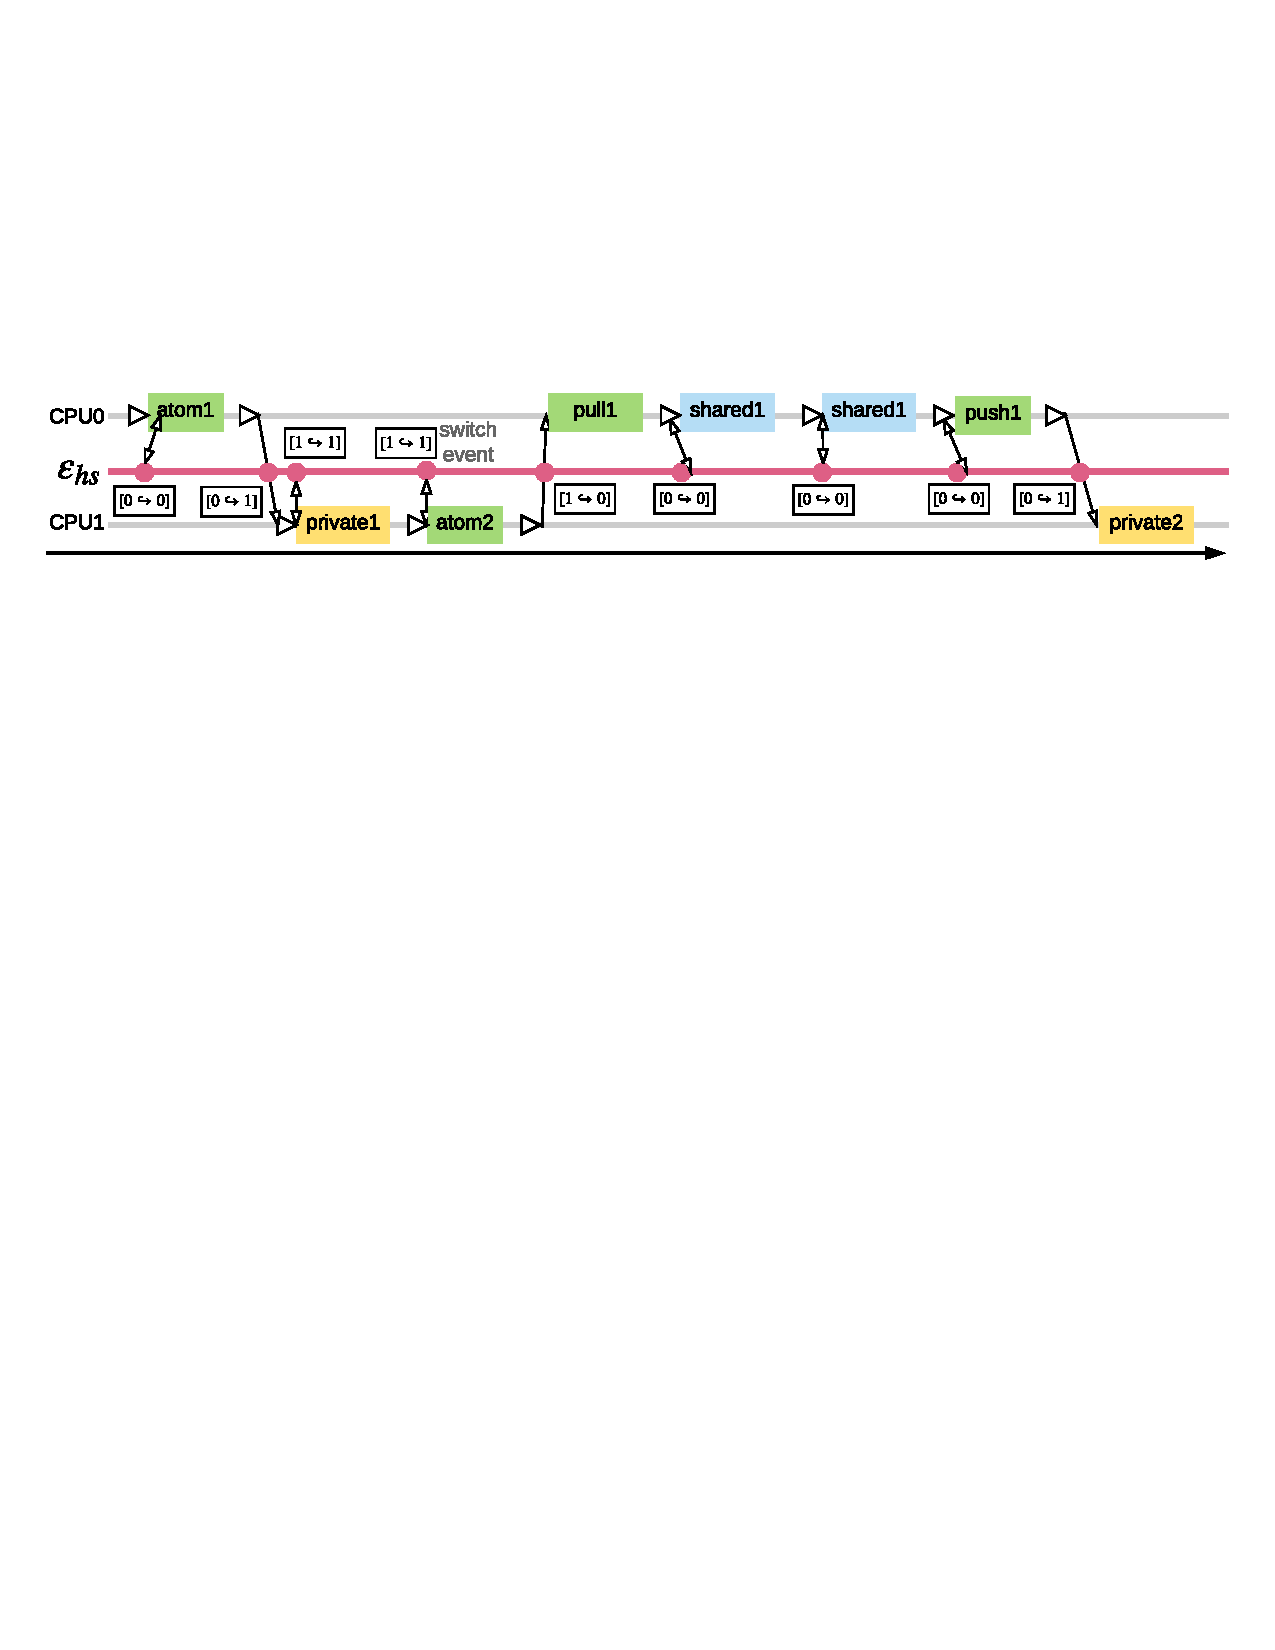
\includegraphics[scale=.52]{figs/machine2}
\vspace{-5pt}
\]

\noindent
The log recorded by this execution is as follows
(a switch from CPU $i$ to $j$ is denoted as $i\switch j$):\vspace{-5pt}
%%%
\[
\begin{footnotesize}
\begin{array}{l}
\!\!\!\!\![\event{0\switch 0, 0.atom_1,  0\switch 1, 1\switch 1,}
\event{1\switch 1, 1.atom_2, 1\switch 0, 0\switch 0,  0\switch 1}]
\end{array}
\end{footnotesize}
\vspace{-5pt}
\]

The behavior of running a program $P$
over this model with a hardware scheduler $\hardoracle$
is denoted as $\mach{hs}(P,\hardoracle)$.
Let $\ectxtc_{hs}$ represents the set of all possible hardware
schedulers. Then we define the whole-machine semantics.
{\small \[
\sem{hs}{P} = \{ ~ \mach{hs}(P,\hardoracle) ~ \mid ~ \hardoracle \in \ectxtc_{hs} ~ \}
\vspace{-15pt}
\]}

\ignore{The machine model with hardware scheduler is denoted as $(\mach{hs}, \hardoracle)$,
to indicate that it is parametrized over all possible $\hardoracle$.}

\noindent
Note that this is a special case of the definition in Sec.~\ref{sec:overview}
for the whole-machine semantics of a concurrent layer machine, where the 
active set is the set of all CPUs.
To ensure correctness of this machine model with respect to the hardware machine model,
we prove that $\mach{x86mc}$ \emph{contextually refines} the new model.
Before we state the property, we first define the notion of
\emph{contextual refinement} formally.

\begin{definition}[Contextual Refinement]
\label{def:mach:refine}
We say layer $L_0$ 
\emph{contextually refines}
layer $L_1$ (written $\forall P, \sem{L_0}{P}\machrel \sem{L_1}{P}$),
iff, for any $P$ that 
does not go wrong 
on $\machx_{L_1}$ under any configuration, (1)~$P$ does not go wrong on $\machx_{L_0}$
under any configuration;
and (2)~any observable behavior of $P$ on $\machx_{L_0}$
under some configuration is also observed on $\machx_{L_1}$
under some (possibly different) configuration.
\end{definition}

\begin{lemma}[Correctness of the hardware scheduler model]\vspace{-3pt}
\label{lemma:hs}
\begin{small}
$$\forall P, \sem{x86mc}{P}\machrel \sem{hs}{P}$$
\end{small}
\vspace{-10px}
\proof[Proof Sketch]
For any interleaved execution on $\machx_{x86mc}$, we construct
a corresponding hardware scheduler on $\mach{hs}$.

\ignore{
Given an observable execution behavior of $P$ running on
$\machx_{x86mc}$, we can construct a particular hardware scheduler
$\hardoracle$ encoding the interleaving that produced the behavior.
The resulting behavior $\mach{hs}(P,\hardoracle)$ is then
an element of $\sem{hs}{P}$ by definition.
}

\ignore{\proof
For any $P$ and any possible interleaving on $\mach{hw}$,
there exists a corresponding hardware scheduler $\hardoracle$,
such that $P$ exhibits an equivalent
behavior when it runs on top of $(\mach{hs}, \hardoracle)$.
\qed}
\end{lemma}

\ignore{
Lemma \ref{lemma:hs} ensures that for
any program running on top of the machine $\mach{hw}$, there exists
a hardware scheduler such that the program exhibits an equivalent
behavior when it runs on top of $\mach{hs}$ with the
hardware scheduler.}

\vspace{-5pt}
\subsection{Machine with local copy of shared memory}
The above machine model does not restrict any access to the shared memory.
We therefore abstract the machine model with hardware scheduler into
a new model that enforces well-synchronized accesses to shared memory.

In addition to the global shared memory concurrently manipulated by all CPUs,
each CPU on this new machine model ($\mach{lcm}$) also maintains
a local copy along with a \emph{valid bit}.
The relation between a CPU's local copy and the global shared memory
is maintained through two new \emph{logical} primitives $\code{pull}$ and $\code{push}$.
The $\code{pull}$ operation updates a CPU's local copy to be equal to the shared memory,
marking the local copy as $\code{valid}$ and the shared memory as $\code{invalid}$.
Conversely, the $\code{push}$ operation updates the shared memory
to be equal to the local copy, marking the shared memory
as $\code{valid}$ and the local copy as $\code{invalid}$.
If a program attempts to pull an $\code{invalid}$ shared memory, push
an $\code{invalid}$ local copy, or access an $\code{invalid}$ local copy,
the program goes wrong.
It makes sure that every shared memory access is always performed on
its $\code{valid}$ local copy, thus systematically enforcing valid accesses to the
shared memory.
Note that all of these constructions are completely \emph{logical}, and do not
correspond to any physical protection mechanisms; thus they do not introduce any
performance overhead.

The shared memory updates of the previous example can be simulated 
on $\mach{lcm}$ as follows:\vspace{-5pt}
\[
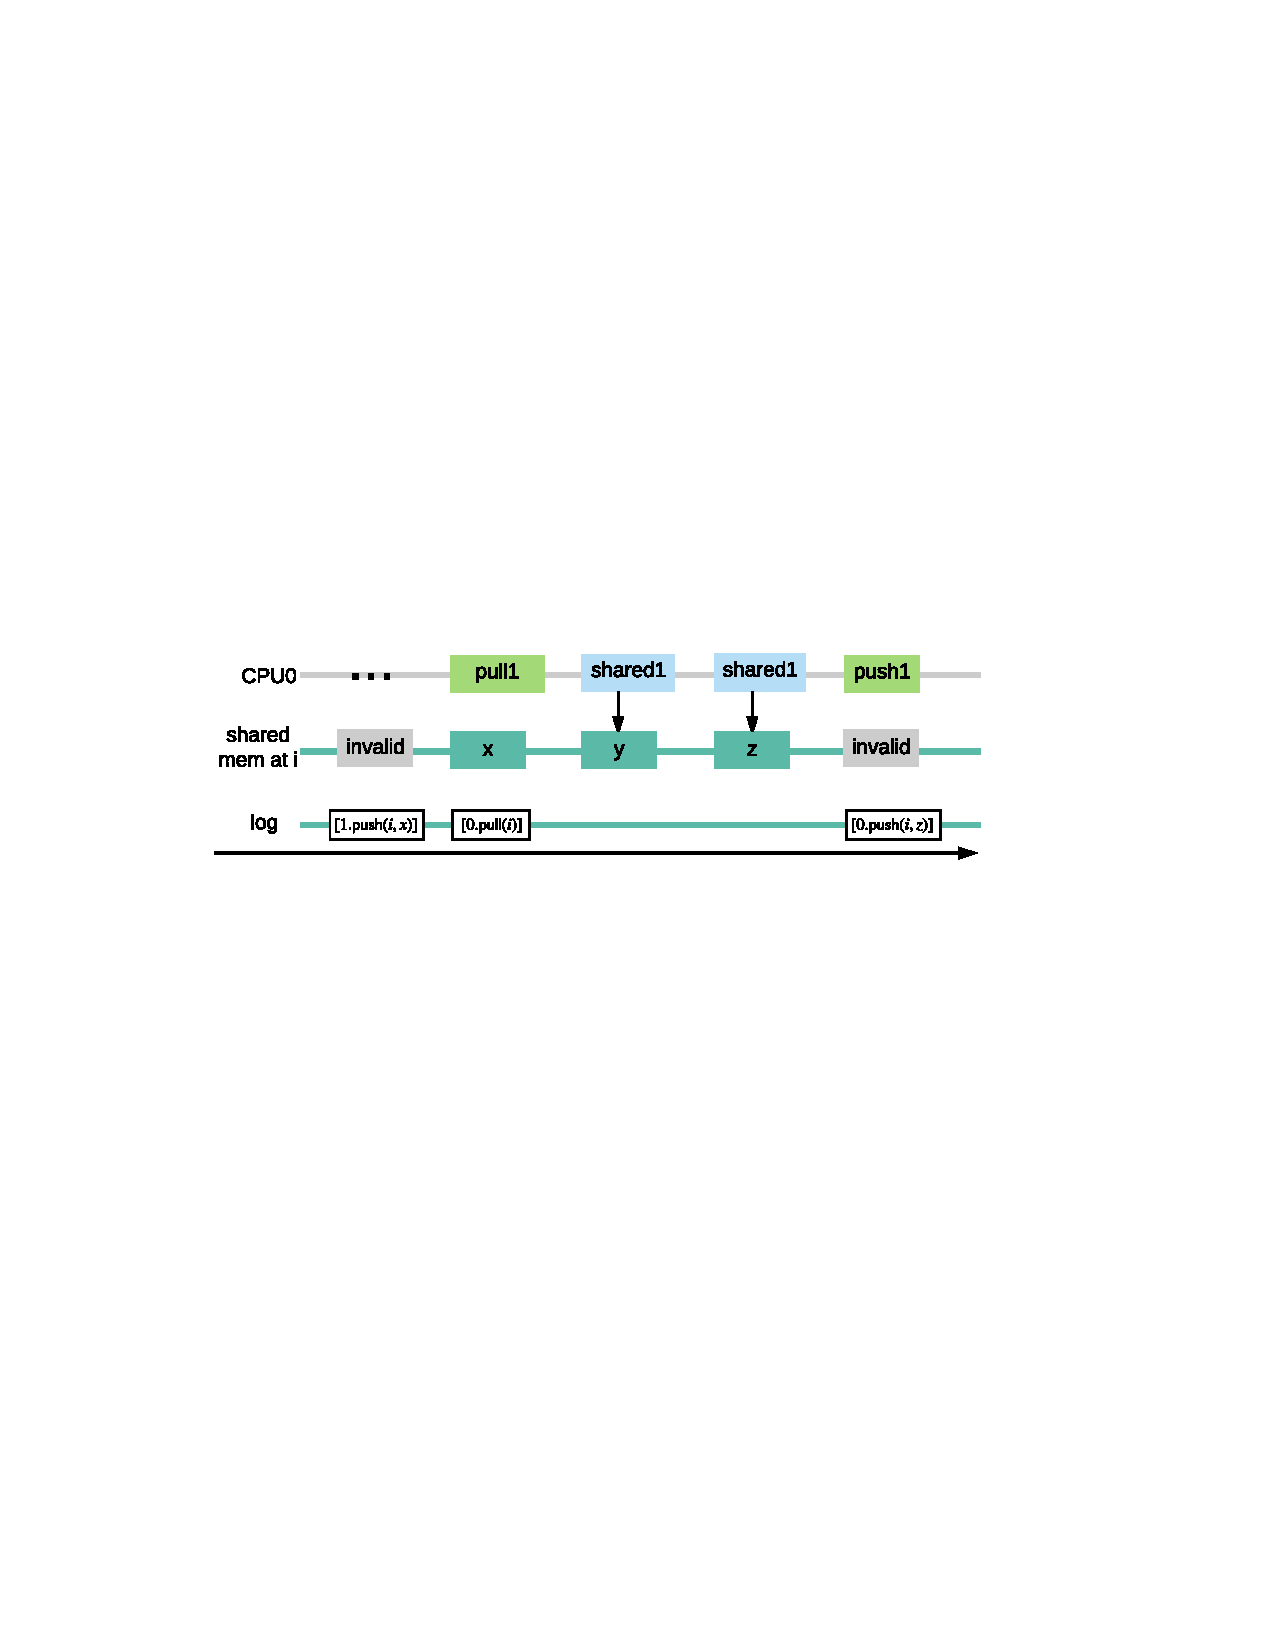
\includegraphics[scale=.6]{figs/machine3}
\vspace{-5pt}
\]

\paragraph{Data-race freedom}
Among the global shared memory and all the local copies, only one can be $\code{valid}$ at any single moment of 
machine execution. 
Therefore, for any program $P$ with a potential \emph{data race}, there exists
a hardware scheduler such that $P$ goes wrong on $\mach{lcm}$.
By showing that a program $P$ is safe (never goes wrong) on $\mach{lcm}$
for \emph{all possible} hardware schedulers, we guarantee that $P$ is data-race free. 

It remains to show that $\mach{lcm}$ is correct with
respect to the previous machine model $\mach{hs}$
with the $\ectxtc_{hs}$.
\begin{lemma}[Correctness of the local copy model]\vspace{-2pt}
{\small \[
\forall P, \sem{hs}{P}\machrel \sem{lcm}{P}\]}
\vspace{-20pt}
%%%
\ignore{
\[\forall \hardoracle, (\mach{hs}, \hardoracle) \machrel 
(\mach{lcm},\hardoracle)\]
}
\ignore{\[\forall P\ \hardoracle, \machbe{P}{\mach{hs}}{\hardoracle}\machrel 
\machbe{P}{\mach{lcm}}{\hardoracle}\]
\proof
For any possible $\hardoracle$, if the program $P$ is safe on $\mach{lcm}$,
then the observable behavior of $P$ on $\mach{lcm}$ is equivalent to
the behavior of $P$ running over $\mach{hs}$.
\qed}
\end{lemma}

\subsection{Partial machine with environment context}

Although $\mach{lcm}$ provides a way to reason about shared memory operations,
it still does not have much support for CPU-local reasoning.
To support modular verification, the machine model should provide
a way to reason about programs on each CPU locally by specifying
expected behaviors of the context programs on other CPUs. The model
should then provide a systematic
way to link the proofs of different local components together to form a global
claim about the whole system. To this purpose, we introduce a partial
machine model $\mach{pt}$ that can be used to reason about the
programs running on a subset of CPUs, by
parametrizing the model over the behaviors of an \emph{environment context}
(\ie, the rest of the CPUs).

We call a given local subset of CPUs the \emph{active CPU set} 
(denoted as $A$).
\ignore{, while all other CPUs are called the 
\emph{context CPU set}.
 of $A$
(denoted as $\overline A$).}
The partial machine model is configured with an active CPU set,
and it queries the environment context whenever it reaches a switch point
that attempts to switch to a CPU outside the active set.

\vspace{-2pt}
\paragraph{Environment context}
of $A$ in this machine model 
is denoted as $\ectxt{pt,A}$.
Each environment context $\oracle_{pt(A)}\in\ectxt{pt,A}$
is a \emph{response function},
which takes the current log 
and returns a list of events from the context programs (\ie, those outside of $A$) 
that is guaranteed to satisfy some invariant.
In other words, response function simulates the observable behavior 
of the context CPUs, and the invariant states the assumptions being 
made over the context.
The hardware scheduler
is also a part of the environment context,
\ie, the events returned by the response function include
switch events. The execution of CPU 0 in the previous example can be simulated
with a $\oracle_{pt(\set{0})}$.
\ignore{$\oracle_{\overline{\set{0}}}$
(\ie, $\oracle_{\set{1}}$, since there are only two CPUs).}\vspace{-2pt}
\[
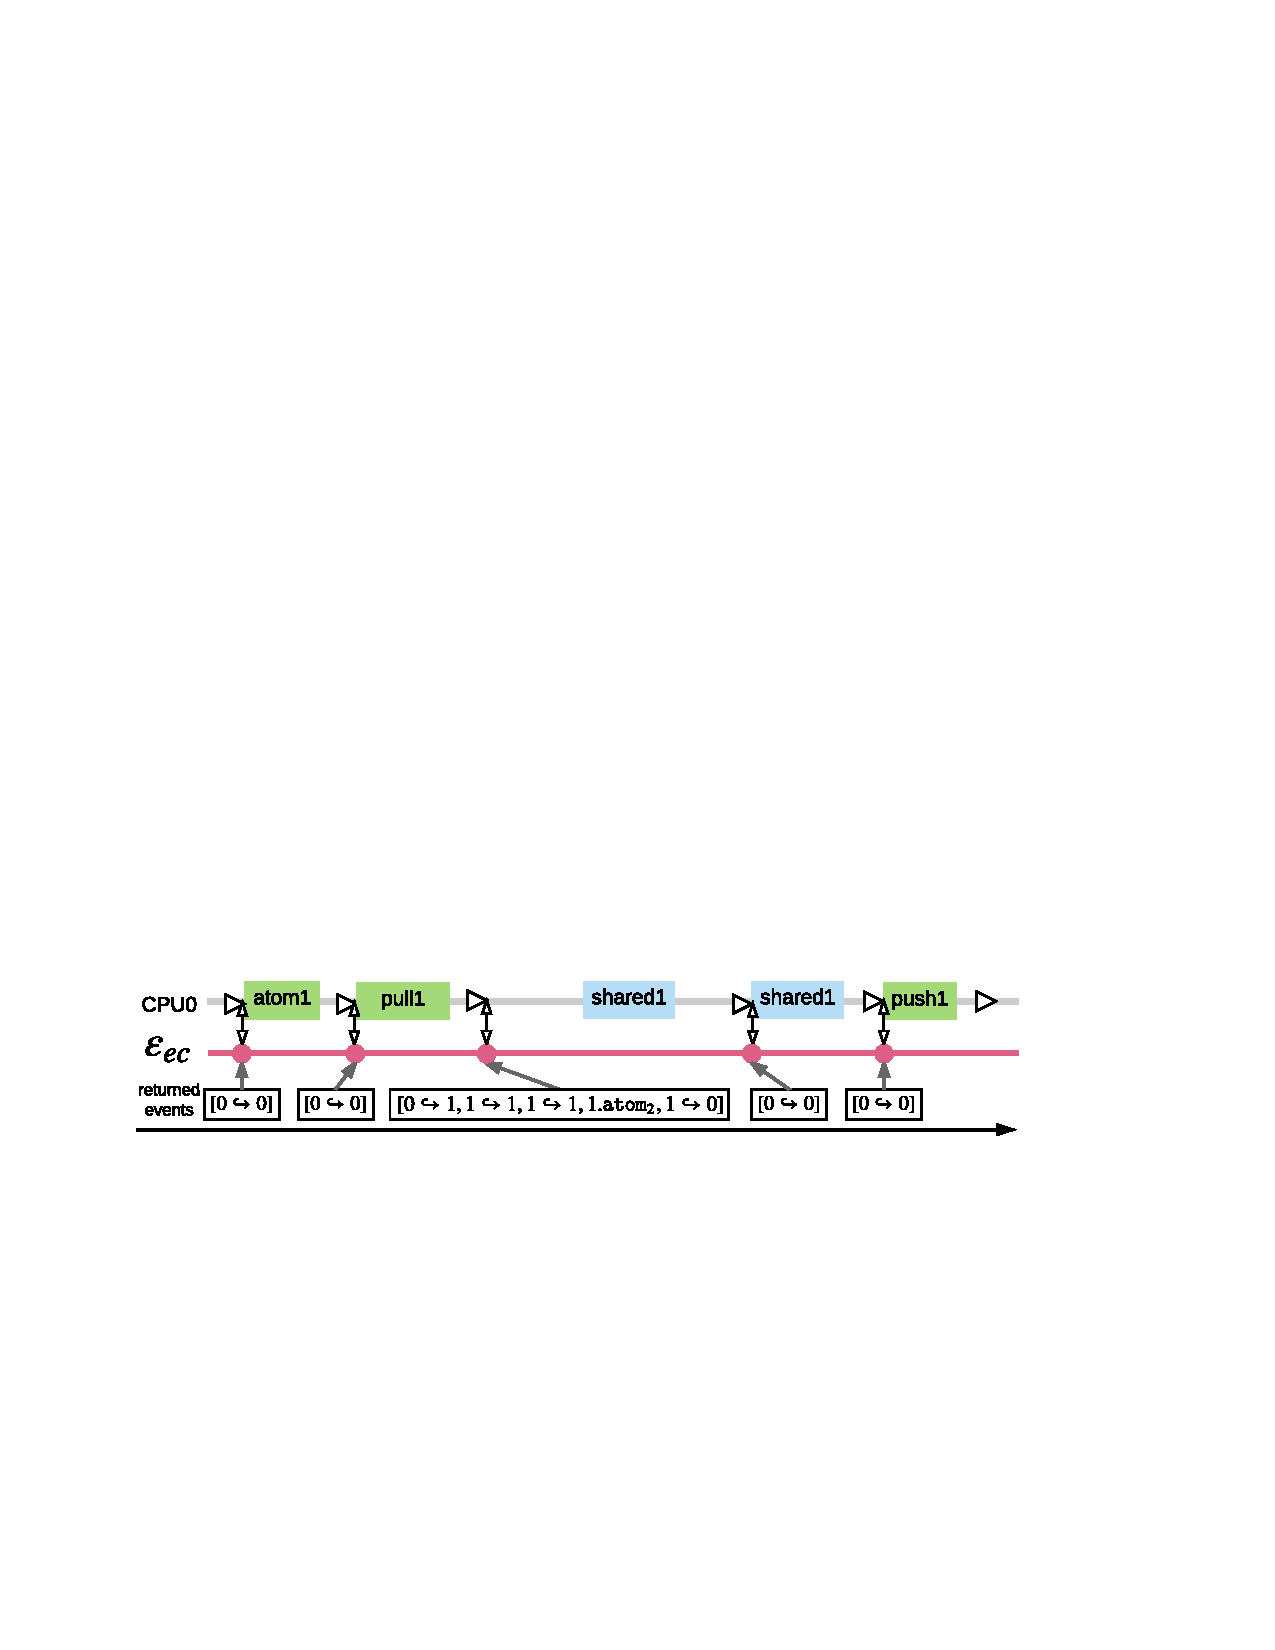
\includegraphics[scale=.53]{figs/machine4}
\vspace{-3pt}
\]

\ignore{The environment context $\oracle_{\set{1}}$
generates the event list $[\event{0\switch 1},\event{1\switch 1},\event{1\switch 1}, \event{1.atom_2}, \event{1\switch 0}]$
at the third \intptext.}

\paragraph{Composition of partial machine models}
Suppose we have verified that two programs, separately running with two 
\emph{disjoint} active CPU sets $A$ and $B$, produce event lists
satisfying invariants $\inv_A$ and $\inv_B$, respectively.
If $\inv_A$ is consistent with the environment context invariant
of $B$,\ignore{(\ie,  $\ectxt{pt,B}$)\ronghui{Do we need this i.e. ?},}
and $\inv_B$ is consistent with the environment context invariant of 
$A$,\ignore{ (\ie, $\ectxt{pt,A}$),}
then we can compose the two separate programs into a single program
with active set $A \cup B$.
This combined program is guaranteed to produce event lists
satisfying the combined invariant $\inv_A \wedge \inv_B$.
Formally, using the whole-machine semantics definition from
Sec.~\ref{sec:overview}, we express this composition as a contextual 
refinement.

\begin{lemma}[Composition of partial machine models]\vspace{-2pt}
\label{lemma:compose}
{\small \[\forall P, \sem{pt(A\cup B)}{P}\machrel \sem{pt(A)}{P} \cap \sem{pt(B)}{P}\quad \text{if } A \cap B = \emptyset\]}
\vspace{-17pt}
\ignore{
\[
\begin{array}{l}
\forall \oracle_{A}\  \oracle_{B}\
\oracle_{\overline{A\cup B}},\\
(\mach{pt},
\oracle_{\overline{A\cup B}})_{A\cup B}
= (\mach{pt},
\oracle_B
\cup \oracle_{\overline{A\cup B}})_A \bigcap
(\mach{pt},
\oracle_A \cup \oracle_{\overline{A\cup B}})_B
\end{array}
\]
}
\ignore{
\proof
If the environment contexts of program $P$ running on $A$ and $B$ are consistent,
then it is equivalent to running $P$ on $A\cup B$ directly. 
\qed}
\end{lemma}

After composing the programs on all CPUs, the context CPU set becomes
empty, and the composed invariant holds on the whole machine.
Since there is no context CPU, the environment context is
reduced to the \emph{hardware scheduler}, which only generates the
switch events. In other words, letting $C$ be the entire set of CPUs
on the machine, we have that $\ectxt{pt,C} = \ectxtc_{hs}$.  By
showing that this \emph{composed machine} with the entire CPU set $C$
is refined by $\mach{lcm}$, the proofs can be propagated down to the
multicore hardware model.

\begin{lemma}[Correctness of the composed total machine]
{\small \[\vspace{-10pt}\forall P, \sem{lcm}{P}\machrel \sem{pt(C)}{P}\vspace{-10pt}\]}
\ignore{
\[
\forall \hardoracle,
(\mach{lcm}, \hardoracle)
\machrel 
(\mach{pt},\hardoracle)\]
}
\ignore{
\[
\forall P\ \hardoracle\ \inv,
\machbe{P}{\mach{lcm}}{\hardoracle}
\machrel 
\machbe{P}{\mach{pt}}{\hardoracle,\inv}\]
\proof
For any given $\hardoracle$, the only difference between two machine models is that
$\mach{partial}$ introduces the invariant $\inv$.
\qed
}
\end{lemma}

\subsection{CPU-local machine model}
\label{subsec:spec:seq}
If we focus on a single active CPU $i$,
the partial machine model is like a \emph{local} machine
with an environment context representing all other CPUs. However,
in this model there is a {\intptext} before each instruction,
so program verification still needs to handle many unnecessary 
interleavings (\eg, the ones between private operations).
In this subsection, we introduce a CPU-local
machine model (denoted as $\mach{loc}$) for a CPU $i$, in which {\intptext}s
only appear before atomic or $\code{push}$/$\code{pull}$ operations.
The {\intptext}s before shared or private operations
are removed via two steps: \emph{shuffling} and \emph{merging}.

\paragraph{Shuffling {\intptext}s}
In $\mach{loc}$, we introduce a \emph{log cache}~--- for
the {\intptext}s before shared and private operations,
the query results from the environment context
are stored in a temporary log cache.
The cached events are applied to the logical log
just before the next atomic or $\code{push}$/$\code{pull}$ operation.
Thus, when we perform shared or private operations,
the observations of the environment context are delayed
until the next atomic or $\code{push}$/$\code{pull}$ operation.
This is possible because a shared operation can only be performed
when the current local copy of shared memory is valid, meaning that 
no other context program can interfere with the operation.

\paragraph{Merging {\intptext}s} Once the {\intptext}s are shuffled properly,
we merge all the adjacent {\intptext}s together.
When we merge {\intptext}s, we also need to merge 
the switch events generated by the environment context.
For example, the change of {\intptext}s for the previous example
on CPU-local machine is as follows: 
\[
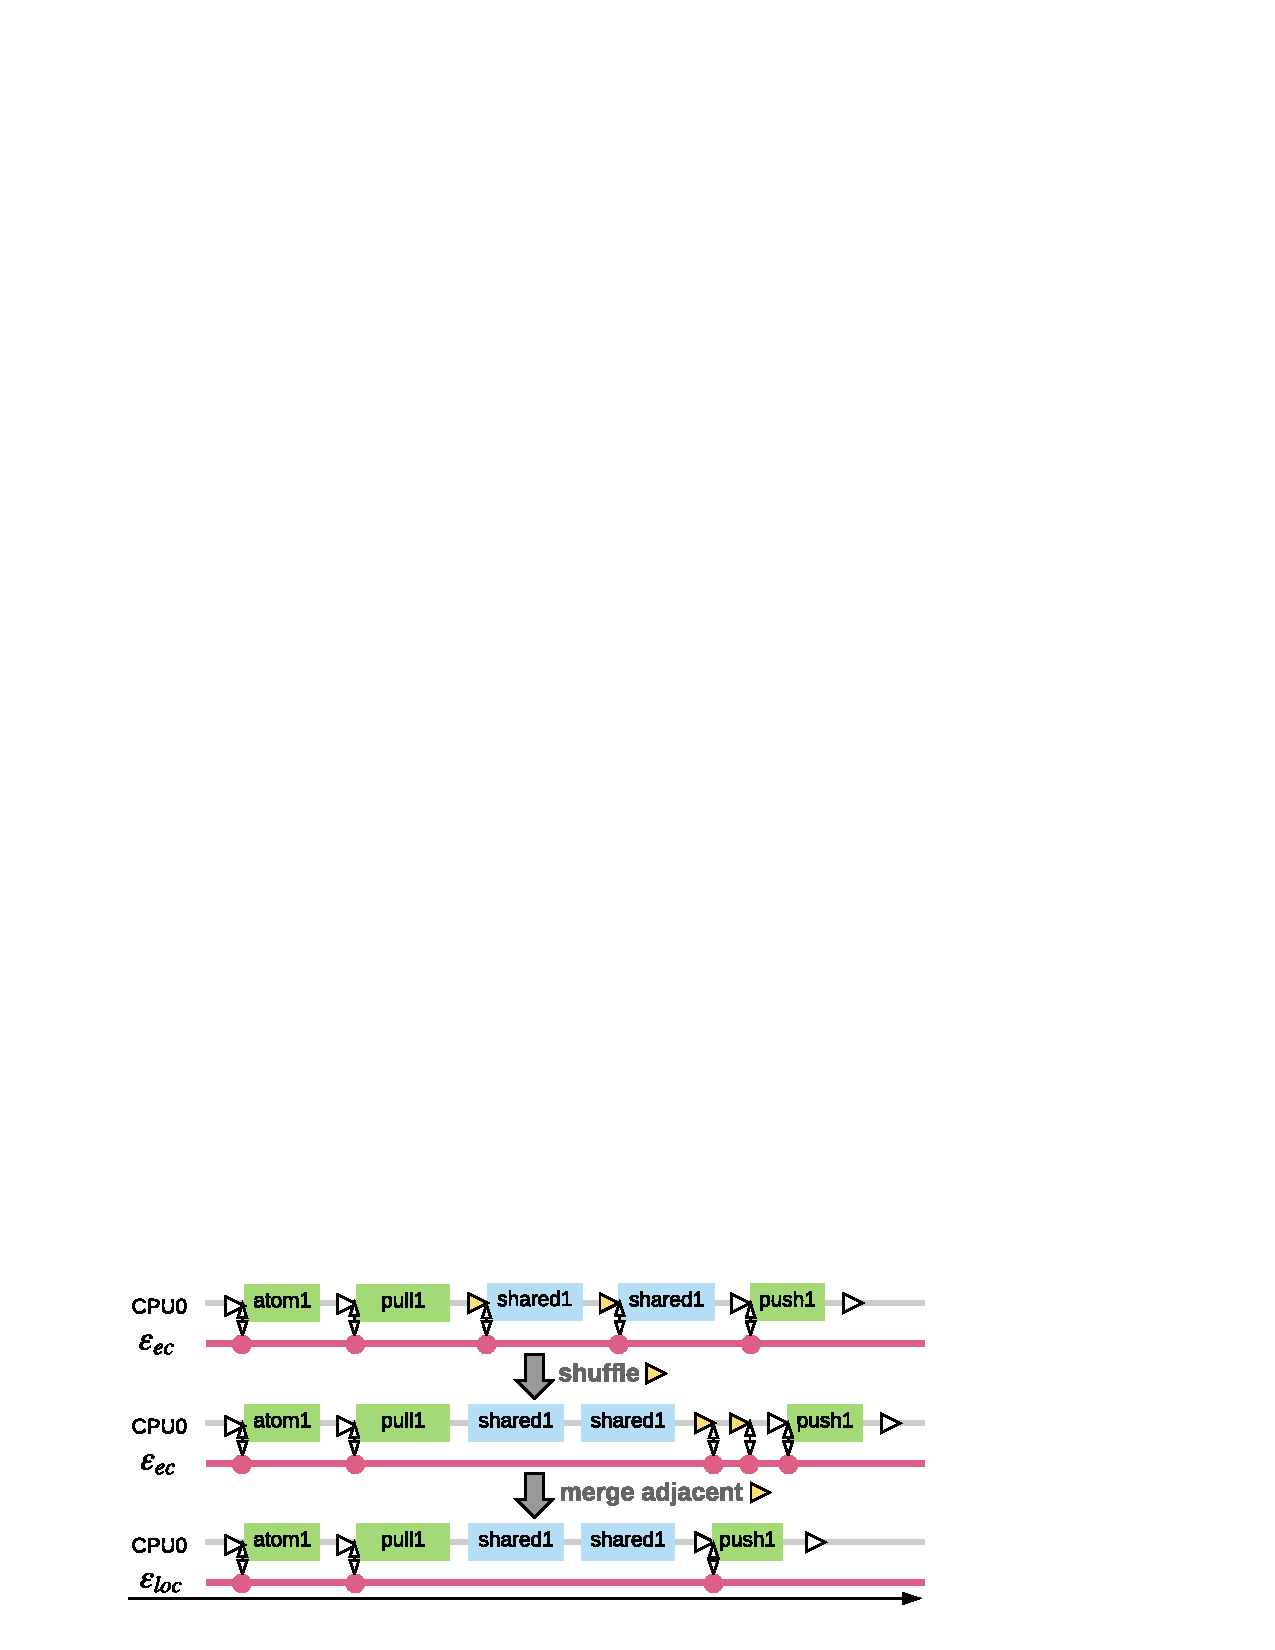
\includegraphics[scale=.57]{figs/machine5}
\]

\begin{lemma}[Correctness of CPU-local machine model]
{\small \[\forall P, \sem{pt(\set{i})}{P}\machrel \sem{loc(\set{i})}{P}\]}
\vspace{-23pt}

\ignore{
\[
\forall \oracle_{\overline{\set{i}}},
\exists \oracle'_{\overline{\set{i}}},
(\mach{pt},\oracle_{\overline{\set{i}}})_{\set{i}}
\machrel 
(\mach{loc},\oracle'_{\overline{\set{i}}})_{\set{i}}
\]
}
\ignore{\[
\begin{array}{l}
\forall P\ \oracle_{\overline{\set{i}}}\ \inv_{\set{i}},
\exists \oracle'_{\overline{\set{i}}},\\
\machbe{P}{\mach{pt}}{\oracle_{\overline{\set{i}}},  \inv_{\set{i}}}
\machrel 
\machbe{P}{\mach{loc}}{\oracle'_{\overline{\set{i}}}, \inv_{\set{i}}}
\end{array}
\]
\proof
Shuffling and merging {\intptext}s  are valid.
\qed}
\end{lemma}

Finally, we obtain the refinement relation from the multicore
hardware model
to the CPU-local machine model by composing
all of the refinement relations together (\cf Fig.~\ref{fig:spec:chain}).
We introduce and verify the {\mCTOS} kernel on top of the CPU-local machine
model $\mach{loc}$. The refinement proof guarantees that the proved properties can be
propagated down to the multicore hardware model $\mach{x86mc}$.





\ignore{
\newman{Copied from the overview section. I will merge them into this
section somehow.}
\subsection{Defining abstraction layers}

We define a concurrent
layer interface $L$ using three components: a collection of
\emph{private objects}, a collection of \emph{atomic objects}, and the
invariants which the atomic and private objects must satisfy at any
point of the execution.  These three components define a {\em logical}
view of a subset of the kernel code and extend an x86-like assembly
machine ($\machx$) with an abstract specification of that code. 

A {\em private object} is the abstraction of private date owned by a
particular thread (or process or CPU). It consists of an
\emph{abstract state} (serving as the abstraction of the underlying
private memory), and a collection of primitives (serving as the
specifications of the methods manipulating that piece of the private
memory). Fig.~\ref{fig:spec:object} shows how to build private
objects.

An {\em atomic object} is the abstraction of shared memory. All of
its methods/primitives are atomic.

As shown in Sec.XXX, the sequential machine model contains a
\emph{small} set of atomic objects, which generates a single event and
the object itself is constructable by replaying the logical log.

Figure~\ref{fig:spec:object} shows how to build atomic objects based
on the atomic objects, private objects, and the shared memory at
underlay.  Since the shared memory accesses are modeled using
\emph{local copy}, the \code{push/pull} operations have to be
synchronized using underlay's atomic objects.  The verification of
functions accessing shared data inside the kernel is a procedure to
show that all shared memory accesses are well-synchronized and its
invocation can be viewed as atomic.

For example, the physical page allocator scans the \emph{shared}
allocation table and returns the first free page.  Its accesses to the
shared table are protected by \emph{atomic lock objects}, such that
its \code{push/pull} operations are safe to execute.  By showing that
the allocator implementation satisfy the specification, which
generates a single \code{palloc} event, an atomic allocator object is
introduced and can be used to reason about other kernel modules at
higher layers (\cf Sec.\ref{sec:base:memm}).

We will use $\mach{L}$ to denote the resulting abstract machine for
each layer interface $L$





\paragraph{Layer invariant}
Each abstraction layer specifies a predicate
on the private objects' abstract states
and the logical log,
which is the invariant $\inv_{\set{i}}$ hold for the execution on CPU $i$
(\cf Sec.XXX).
We have to show that this invariant $\inv_{\set{i}}$ is preserved
by all primitives of private objects and atomic objects.
The proofs for atomic  objects also rely on the
invariant of the context CPUs (\ie, $\inv_{\bar{\set{i}}}$).

In previous verification efforts, even for private objects,
proving invariants has typically been challenging~\cite{klein2009sel4},
especially that the invariants might be temporarily violated within the function body.
For example, adding a new node to a doubly-linked list
temporarily violates invariants that the list is well formed.

However, in our layered approach,
we do not have to set up the all the invariants at a single step.
Take the thread queue (implemented as doubly-linked list) in C2 kernel as an example.
When verifying the concrete implementation, we do not pose the well-formedness invariant
over the queue at that layer.
We only prove the invariant after the queue and its operations be introduced as a private object and the primitives.
In this way,
since the abstract primitives are atomic,
there is no longer a point in the execution
at which the invariants have to be temporarily violated.




\subsection{Contextual Refinement}
The contextual refinement relation between
the two layers (one with concrete implementation and the other
with the private and atomic object) ensures that any kernel/user context code 
(\ie, threads on other CPUs and other modules on the same CPU)
linking with the more abstract layer retains an
equivalent behavior when linking with the corresponding
concrete implementation running on the layer.

\paragraph{Contextual refinement for private objects}
As shown in Fig.~\ref{fig:spec:object},
to establish the contextual refinement relation
between concrete memory and the private object,
we use memory permissions~\cite{leroy08} at the higher layer
to prevent the context code
from accessing the private memory.
Note that these permissions do \emph{not}
correspond to a physical protection mechanism,
but instead are entirely logical:
they ensure that the higher-level abstract machine
gets stuck whenever it executes
code that directly accesses this private memory without going through the provided
primitives. By proving that our kernel is safe (it will not go wrong),
we guarantee that this situation will not happen.

\paragraph{Contextual refinement for atomic objects}
To establish the contextual refinement relation
for atomic objects, the main proof body is about the invariants proof.
We have to show that for any environment context $\oracle_{\bar{\set{i}}}$
that satisfy the context invariant $\inv_{\bar{\set{i}}}$.
Thus, the environment context linked with CPU $i$'s atomic object
is equivalent to the one linked with the concrete implementation,
where interleaving might happen within the function body.

\paragraph{Layer refinement}


The first layer \emph{PreInit} (\ie, $L_0$)
is based on the \emph{sequential machine model} $\mach{s}$.
As shown in Fig.\ref{fig:spec:refine_layer},
kernel modules
are verified as a stack of layers
building 
on top of the $\mach{s}$.
Although the layers are built
on behave of a particular $\text{CPU}_i$,
layers at other CPUs are symmetric.
After the scheduler module is verified,
we move one step forward
and decompose the execution on $\text{CPU}_i$
into a collection of \emph{per-thread execution}.
By introducing the \emph{software scheduler}
$\oracle_{ss}$ (\ie, reflecting the scheduling algorithm),
multi-threads execution on the same CPU 
can be composed similarly to the multi-core composition
(\cf Sec.~\ref{sec:base:procm}).
Thus, user programs can be verified
locally using the atomic specifications of kernel's
system calls,
and be composed using our framework.

}


